In my thesis work, we have been focusing on assessing someone's risk of disease based on DNA data. Except for somatic mutations, DNA data do not change over lifetime so that we could, in theory, assess someone's genetic risk of disease at birth. Thus, this could have potentially large implications in disease prevention \cite[]{mavaddat2015prediction,pashayan2015implications}.
As an example, about 12\% of women in the general population will develop breast cancer sometime during their lives \cite[]{desantis2016breast}. By contrast, a recent large study estimated that about 72\% (95\% CI: 65\%-79\%) of women who inherit a harmful BRCA1 mutation and about 69\% (95\% CI: 61\%-77\%) of women who inherit a harmful BRCA2 mutation will develop breast cancer by the age of 80 \cite[]{kuchenbaecker2017risks}. 
In 2013, Angelina Jolie announced that she had undergone a preventative double mastectomy, because she had a family history of breast cancer and was carrying a harmful BRCA1 mutation.
Thereby, DNA data can help identify individuals who are at high-risk for some diseases in order to target preventive actions.

In this introduction, we first introduce the context of our research and the type of data we work with. Then, we present the statistical methods that are widely used in our field, and how the field has moved from association testing to prediction. Finally, we present the main statistical and computational challenges that has driven our research, which has resulted in two peer-reviewed papers and another submitted paper currently available as a preprint.

\section{Context}

Today, clinical risk prediction for common adult-onset diseases often relies on basic demographic characteristics, such as age, gender and ethnicity; basic health parameters and lifestyle factors, such as body mass index, smoking status, alcohol consumption and physical exercise habits; measurement of clinical risk factors linked to disease onset, such as blood pressure levels, blood chemistries or biomarkers indicative of ongoing disease processes; ascertainment of environmental exposures, such as air pollution, heavy metals and other environmental toxins; and family history \cite[]{torkamani2018personal}.
Routine genetic profiling is absent from this list, often relegated to use only when testing clarifies individual-level risks in the context of a known family history for some common adult-onset
diseases \cite[]{torkamani2018personal}.

\subsection{Different types of diseases and mutations}

How mutations affect diseases depends on their effect sizes and on their allele frequencies (Figure \ref{fig:rare-common}).
For example, harmful BRCA mutations are highly penetrant mutations, i.e.\ that most women carrying these mutations will develop breast cancer. Many mutations with large effect sizes have been identified and are referenced in an online database \cite[]{hamosh2005online}. 
Those mutations are often very rare; either they are associated with some very rare disease or they explain only a small proportion of common diseases incidence \cite[]{anglian2000prevalence}.
In this work, we focus on common diseases (e.g.\ breast cancer) and try to predict individuals' disease susceptibility based on common variants; the common disease--common variant hypothesis \cite[]{pritchard2002allelic}. This hypothesis further suggests that such diseases are likely caused by a large number of common variants, each contributing only a small risk and thereby evading negative evolutionary selection \cite[]{salari2012personalized}.
Indeed, selection might be responsible for keeping genetic effect sizes low, since variants of larger effect may be selected against and eventually disappear \cite[]{pritchard2002allelic}.
One common form of variation across human genomes is called a single nucleotide polymorphism (SNP). As indicated by the name, SNPs are single base changes in the DNA.
Genotyping technologies now exists to genotype hundreds of thousands of SNPs at once for around \$50 only. Starting with the \cite{wellcome2007genome}, these new sequencing technologies had led to many genome-wide association studies.%, which we talk about in the next section. From these studies, it was found that effects of common variants that are associated with some disease are typically very small.

\begin{figure}[htb]
\centerline{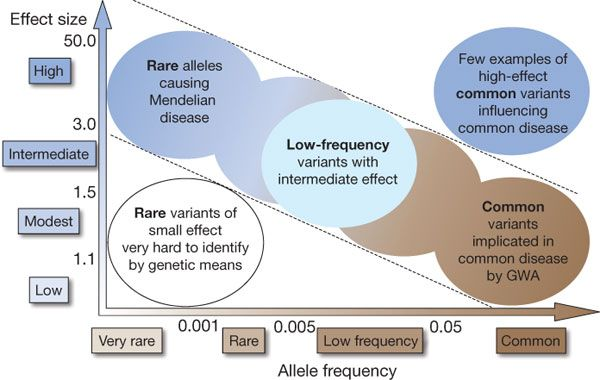
\includegraphics[width=0.7\textwidth]{rare-common.jpg}}
\caption{Feasibility of identifying genetic variants by risk allele frequency and strength of genetic effect (odds ratio). Most emphasis and interest lies
in identifying associations with characteristics shown within diagonal dotted
lines. Source: \cite{manolio2009finding}.}
\label{fig:rare-common}
\end{figure}

\subsection{Genome-Wide Association Studies (GWAS)}

\cite{visscher201710} provide a thorough review of the aims and outcomes of GWAS and \cite{tam2019benefits} talk extensively about the benefits and limitations of GWAS.
The method behind GWAS is simple: test each variant one by one for association with a phenotype of interest.
For a continuous phenotype (e.g.\ height), linear regression is used and, for each SNP $j$, a t-test is performed to look for an association between this SNP and the phenotype of interest ($\beta^{(j)} = 0$ vs $\beta^{(j)} \neq 0$), where
\begin{equation}
y = \alpha_j + \beta_j G_{j} + \gamma_j^{(1)} COV^{(1)} + \cdots + \gamma_j^{(K)} COV^{(K)} + \epsilon~,\label{eq:gwas1}
\end{equation}
$y$ is the continuous phenotype, $\alpha_j$ is the intercept, $G_{j}$ is SNP $j$ with effect $\beta_j$, $COV^{(1)}$, ..., $COV^{(K)}$ are $K$ covariates with effects $\gamma_j^{(1)}$, ..., $\gamma_j^{(K)}$, including principal components and other covariates such as age and gender. Similarly, for a binary phenotype (e.g.\ disease status), logistic regression is used and a Z-test is performed on $\beta^{(j)}$ for each SNP $j$ where
\begin{equation}
\log{\left(\frac{p}{1-p}\right)} = \alpha_j + \beta_j G_{j} + \gamma_j^{(1)} COV^{(1)} + \cdots + \gamma_j^{(K)} COV^{(K)}~,\label{eq:gwas2}
\end{equation}
$p = \mathbb{P}(Y = 1)$ and $Y$ denotes the binary phenotype.

It is well established that principal components of genotype data should be included as covariates in GWAS to account for the confounding effect of population structure \cite[]{price2006principal}. Indeed, principal components of genotype data capture well population structure (as shown in figure \ref{fig:pca}). 
To illustrate the importance of accounting for population structure, consider a dataset where there are 900 Finnish people and 100 Italian people. Because Finnish people are on average taller than Italian people, any SNP with a large difference in allele frequency between these two populations would be flagged as being associated with height, leading to many false positive associations. Thus, adding principal components as covariates aims at preventing those SNPs from being false positive reports.

\begin{figure}[htb]
\centerline{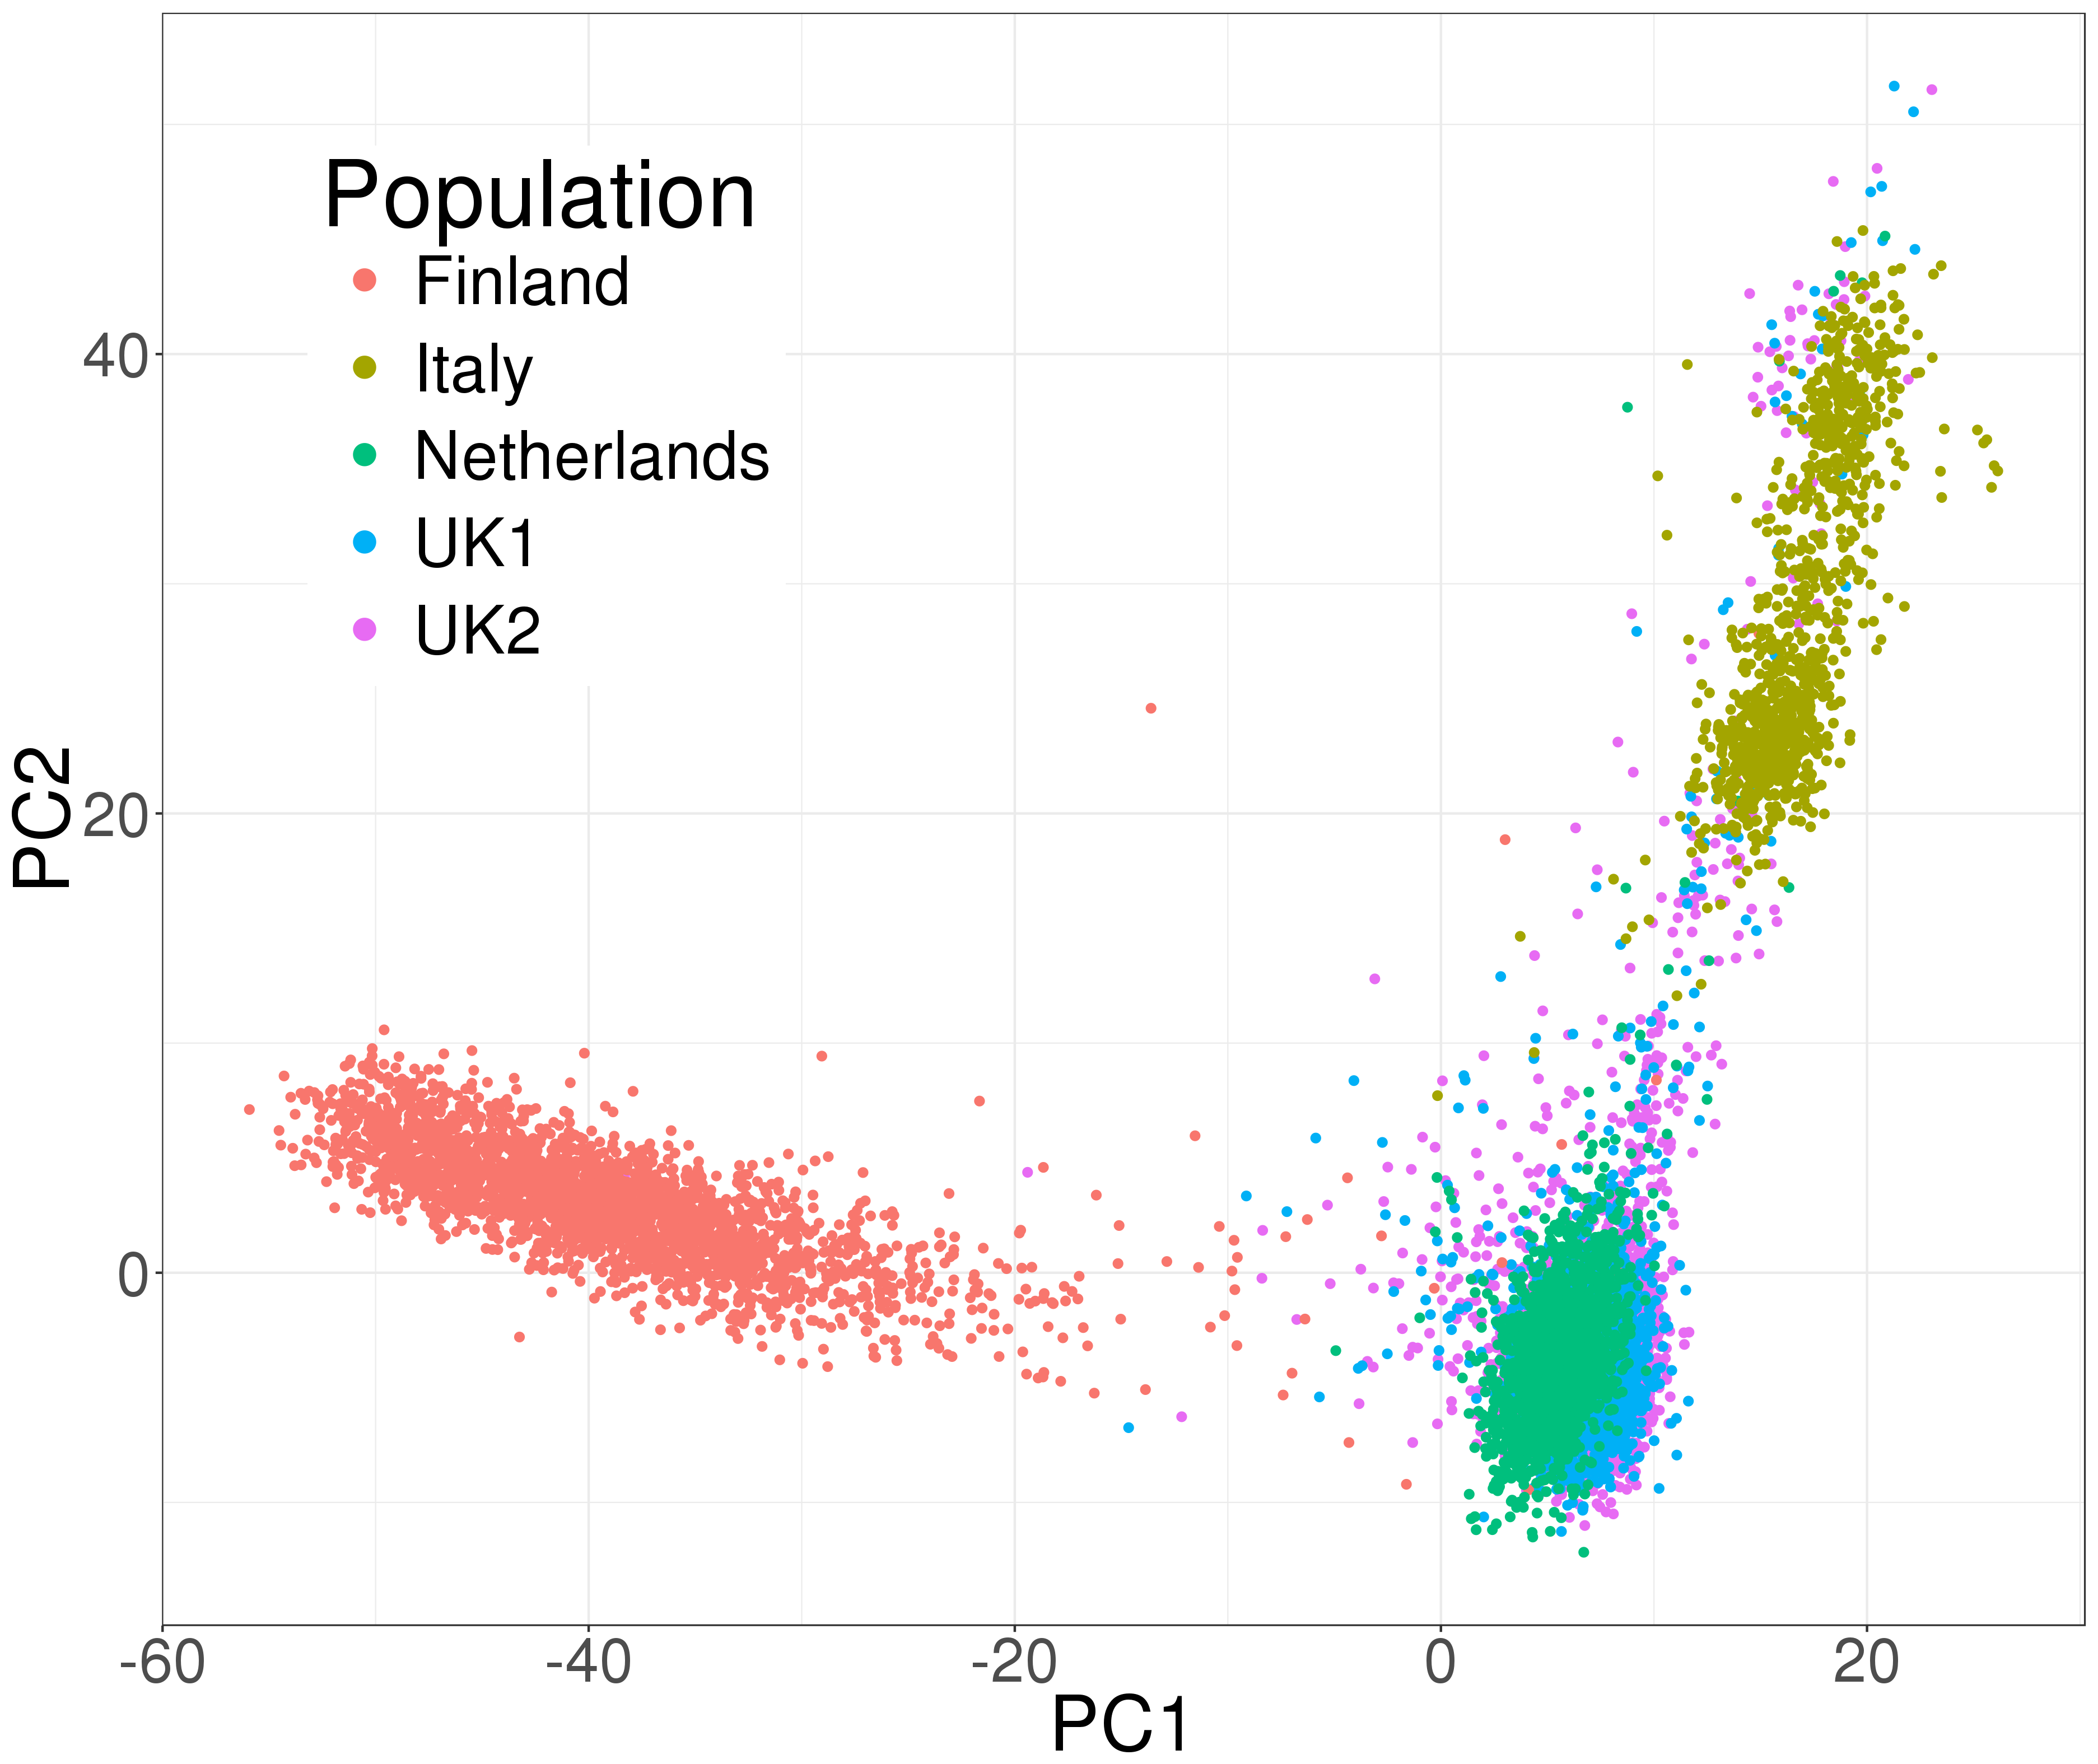
\includegraphics[width=0.6\textwidth]{celiac-pca.png}}
\caption{First two Principal Components of individuals from four European populations. PC1 correlates with latitude while PC2 correlates longitude. Data come from a case-control study for celiac disease \cite[]{dubois2010multiple}.}\label{fig:pca}
\end{figure}

These simple tests can be used only if individuals are not related to one another. If they do, a common practice is to remove one individual from each pair of related individuals. Another strategy is to use Linear Mixed Models (LMM) to take into account both relatedness and population structure; these mixed models have also the potential to increase discovery power in association testing \cite[]{yang2014advantages}.

To date, more than 10,000 strong associations have been reported between genetic variants and one or more complex traits \cite[]{welter2013nhgri}, where ``strong'' is defined as statistically significant at the genome-wide p-value threshold of $5 \cdot 10^{-8}$. This threshold corresponds to a type-I error of 5\%, Bonferroni-corrected for one million independent tests \cite[]{pe2008estimation}. Results of a GWAS are usually reported in a Manhattan plot (Figure \ref{fig:gwas}). 
Manhattan plots show some association peaks (similar to skyscrapers in Manhattan) due to some local correlation between SNPs (Linkage Disequilibrium), with squared correlation roughly inversely proportional to distance between SNPs \cite[]{hudson2001two}.

\begin{figure}[htb]
\centerline{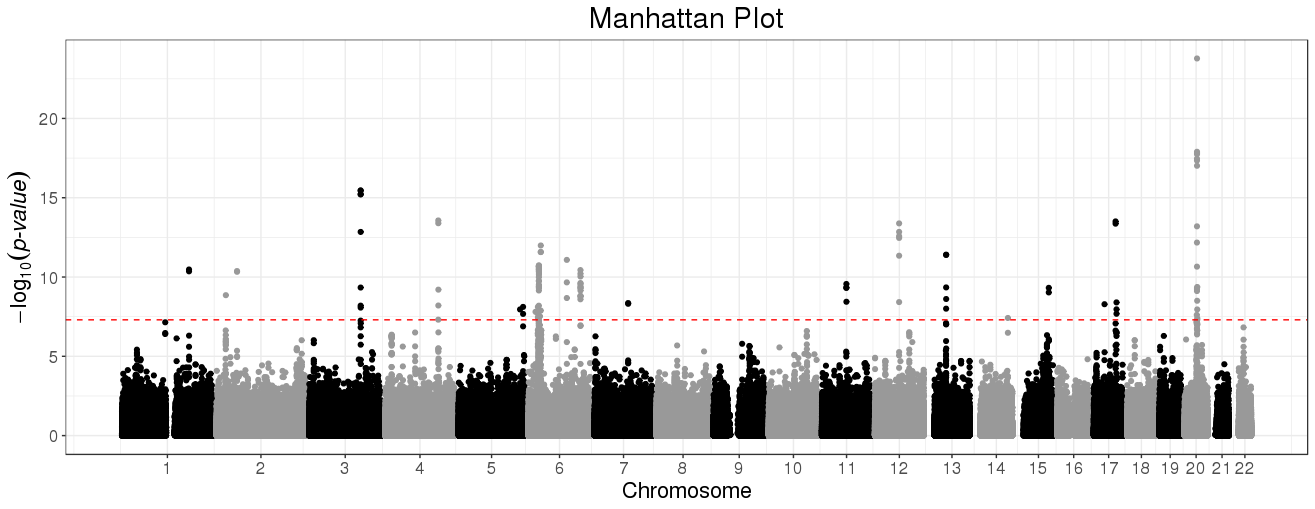
\includegraphics[width=0.95\textwidth]{gwas-height-20K.png}}
\caption{Manhattan plot from a GWAS of height based on 20,000 unrelated individuals from the UK Biobank dataset \cite[]{bycroft2017genome}.}\label{fig:gwas}
\end{figure}


\subsection{GWAS data}

There are mainly three types of individual-level data: genotyped SNPs from genotyping chips, imputed SNPs from reference panels, and Next Generation Sequencing (NGS) data.
Genotyping chips enables a quick and cheap genotyping of 200K to 2M SNPs, mostly focusing on common variants (Minor Allele Frequency (MAF) larger than 1-5\%). From this genotyping, you can get a matrix of $0$s, $1$s and $2$s, counting the number of alternative alleles for each individual (row) and each genome position (column). There are usually few missing values (less than 5\% in total) when using this technology.

Imputation has a different meaning in genetics than in other Data Science fields; it does not refer to filling those 5\% missing values, but instead refers to adding completely new variants that were not genotyped with the chip used. 
Imputation is enabled by the fact that genotypes of unobserved genetic variants can be predicted by haplotypes inferred from multiple observed SNPs (the ones that were genotyped) and haplotypes observed from a fully sequenced reference
panel \cite[]{marchini2010genotype,mccarthy2016reference}.
Imputation now allows to have large genomic datasets such as the UK Biobank: 90M imputed SNPs for each of 500K genotyped individuals who were sequenced at 800K SNPs only \cite[]{bycroft2017genome}.

Finally, NGS (also named Whole Genome Sequencing (WGS)) refers to fully sequenced data over more than 3M variants, including some rare variants. Yet, this technology is still very expensive, with a cost of around \$1000 per genome.
GWAS to date have been based on SNP arrays designed to tag common variants in the genome. These arrays do not cover all genetic variants in the population, and it seems natural that future GWAS will be based on WGS. However, the price differential between SNP arrays and WGS is still substantial, and array technology remains more robust than sequencing \cite[]{visscher201710}. An in-between solution could be to use extremely low-coverage sequencing \cite[]{pasaniuc2012extremely}.

Recently, some national biobank projects have emerged. For example, the UK Biobank has released both genome-wide genotypes and rich phenotypic data on 500K individuals to the international research community \cite[]{bycroft2017genome}.
Yet, it is rare to have access to large individual-level genotype data. 
Most of the time, only summary statistics for a GWAS dataset are available, i.e.\ the estimated effect sizes and p-values for each variant of the dataset (Table \ref{tab:sumstats}). Because of the availability of such data en masse, specific methods using those summary data have been developed for a wide range of applications such as imputation, polygenic prediction and heritability estimation \cite[]{pasaniuc2014fast,vilhjalmsson2015modeling,bulik2015ld,pasaniuc2017dissecting,speed2018sumher}. The craze for such data can be explained by the fact that GWAS individual-level data, sometimes consisting of dozens of different datasets, cannot be easily shared publicly, as opposed to summary data \cite[]{lin2010meta}.
So, modern large GWAS are in fact meta-analyses of many smaller GWAS summary statistics.
Moreover, methods using summary statistics data are usually fast and easy to use, making them even more appealing to researchers.

In this thesis, we have not used NGS data, but we have used genotyped SNPs, imputed SNPs and summary statistics to construct predictive models of disease risk, for many common diseases.

% latex table generated in R 3.5.2 by xtable 1.8-2 package
% Wed Apr  3 17:55:25 2019
\begin{table}[ht]
\caption{An example of summary statistics for type 2 diabetes \cite[]{scott2017expanded}. Generally, effects and p-values are available for all SNPs in the GWAS, where there can be many millions of them \cite[]{asking4more}.}\label{tab:sumstats}
\vspace{0.5em}
\centering
\begin{tabular}{rrccrrrr}
  \hline
Chr & Position & Allele1 & Allele2 & Effect & StdErr & P-value & TotalSampleSize \\ 
  \hline
   5 & 29439275 & T & C & -0.000 & 0.015 & 0.990 & 111309 \\ 
     5 & 85928892 & T & C & -0.008 & 0.031 & 0.790 & 111309 \\ 
    11 & 107819621 & A & C & -0.110 & 0.200 & 0.590 & 87234 \\ 
    10 & 128341232 & T & C & 0.024 & 0.015 & 0.110 & 111309 \\ 
     8 & 66791719 & A & G & 0.069 & 0.120 & 0.560 & 99092 \\ 
    23 & 145616900 & A & G & -0.011 & 0.060 & 0.860 & 19870 \\ 
     3 & 62707519 & T & C & 0.006 & 0.034 & 0.860 & 111308 \\ 
     2 & 80464120 & T & G & 0.110 & 0.057 & 0.062 & 108514 \\ 
    18 & 51112281 & T & C & -0.011 & 0.016 & 0.490 & 111307 \\ 
     1 & 209652100 & T & C & 0.260 & 0.170 & 0.120 & 84836 \\ 
   \hline
\end{tabular}
\end{table}


%%%%%%%%%%%%%%%%%%%%%%%%%%%%%%%%%%%%%%%%%%%%%%%%%%%%%%%%%%%%%%%%%%%%%%%%%%%%%%%%


\section{From GWAS to Polygenic Risk Scores (PRS)}

For thorough guides on how to perform PRS analyses, please refer to \cite{wray2014research,chasioti2019progress,choi2018guide}.

\subsection{A standard way to compute PRS}\label{sec:C+T}

The main method for computing Polygenic Risk Scores (PRS) is the widely used ``Clumping + Thresholding'' (C+T, also called ``Pruning + Thresholding'' in the literature) model based on univariate GWAS summary statistics as described in equations \eqref{eq:gwas1} and \eqref{eq:gwas2}.
Under the C+T model, a coefficient of regression is learned independently for each SNP along with a corresponding p-value (the GWAS part). 

The SNPs are first clumped (C) so that there remains only SNPs that are weakly correlated with each other ($S_\text{clumping}$). Clumping looks at the most significant SNP first, computes correlation between this index SNP and nearby SNPs (within a genetic distance of e.g.\ 500kb) and remove all the nearby SNPs that are correlated with this index SNP beyond a particular threshold (e.g.\ $r^2 = 0.2$, \cite{wray2014research}). 
The clumping step aims at removing redundancy in included effects that is simply due to linkage disequilibrium (LD) between variants (see figures \ref{fig:gwas2} and \ref{fig:gwasLD}). Yet, this procedure may as well remove independently predictive variants in nearby regions.

Thresholding (T) consists in removing SNPs that are under a chosen level of significance (a p-value threshold $p_T$) in order to reduce noise in the score.
In figure \ref{fig:gwas2}, using no threshold corresponds to ``C+T-all''; using the genome-wide threshold of $5 \cdot 10^{-8}$ corresponds to ``C+T-stringent''; generally, many values are tested to choose an ``optimal'' value for this parameter. 

A polygenic risk score is finally defined as the sum of allele counts of the remaining SNPs (after clumping and thresholding) weighted by the corresponding GWAS effect sizes \cite[]{purcell2009common,Dudbridge2013,wray2014research,Euesden2015},
\[\rm{PRS}_i = \sum_{\substack{j \in S_\text{clumping} \\ p_j~<~p_T}} \hat\beta_j \cdot G_{i,j}~,\] where $\hat\beta_j$ ($p_j$) are the effect sizes (p-values) estimated from the GWAS and $G_{i,j}$ is the allele count (genotype) for individual $i$ and SNP $j$.

\begin{figure}[htb]
\centerline{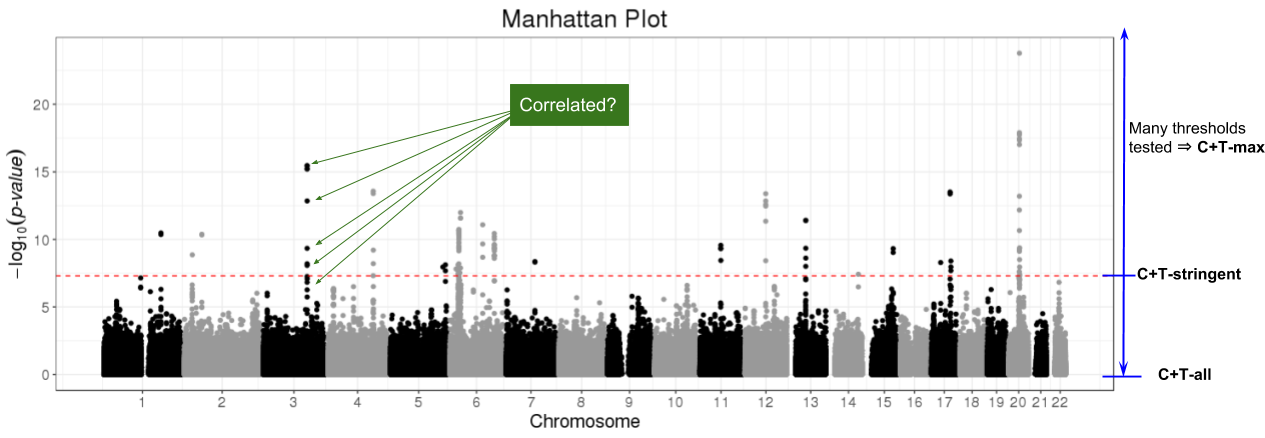
\includegraphics[width=0.95\textwidth]{GWAS2PRS3.png}}
\caption{Illustration of C+T looking at a Manhattan plot from a GWAS of height based on 20,000 unrelated individuals from the UK Biobank dataset \cite[]{bycroft2017genome}. \textbf{\color{clumping}Clumping} removes nearby SNPs that are too correlated with one another because indirect associations due to Linkage Disequilibrium provide only redundant information (see figure \ref{fig:gwasLD}). \textbf{\color{thresholding}Thresholding} includes SNPs if they are significant enough ($p_j < p_T$) in order to reduce noise in the polygenic score.}\label{fig:gwas2}
\end{figure}

\begin{figure}[htb]
\centerline{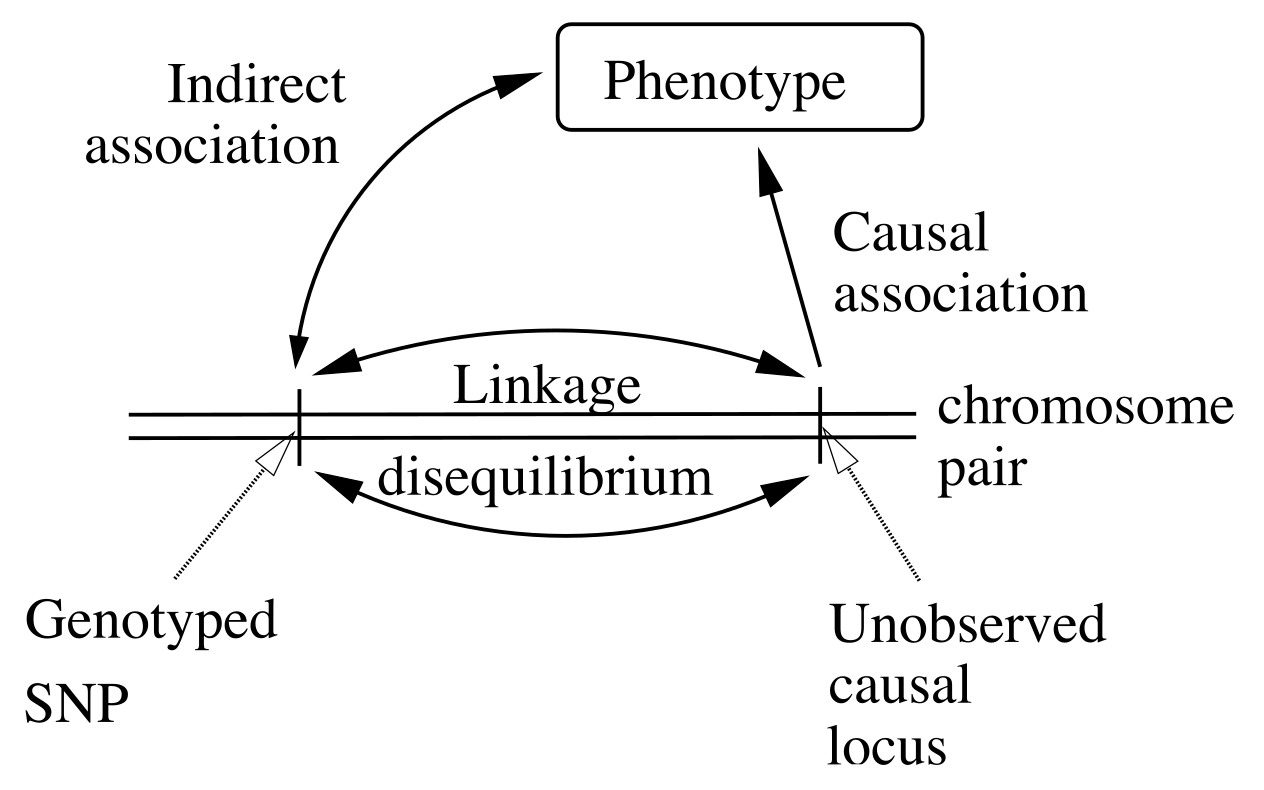
\includegraphics[width=0.5\textwidth]{indirect-association.png}}
\caption{Illustration of an indirect association with a phenotype due to Linkage Disequilibrium between SNPs. Source: \cite{astle2009population}.}\label{fig:gwasLD}
\end{figure}

\subsection{PRS for epidemiology}

Polygenic Risk Scores (PRS) have been used for epidemiology before being used for prediction. The steps for a PRS analysis are illustrated in figure \ref{fig:steps-PRS} and have two goals. 
First, PRS can be used when there is no SNP detected (at $5 \cdot 10^{-8}$) in a GWAS in order to show that there is still a significant polygenic contribution to the phenotype of interest. 
For example, in 2009, a GWAS for Schizophrenia by \cite{purcell2009common} found only a single significantly associated SNP, although this disease is known to be highly heritable. Yet, by constructing a PRS using these GWAS results and testing this polygenic score for association with Schizophrenia in another independent dataset, \cite{purcell2009common} proved that there is a polygenic contribution to Schizophrenia (Figure \ref{fig:epi-PRS}). 
Thus, polygenic analysis methods were central in demonstrating that the first phase of GWAS were underpowered, which propelled the drive for larger sample sizes that is now starting to pay off \cite[]{wray2014research}.

\begin{figure}[htb]
\centerline{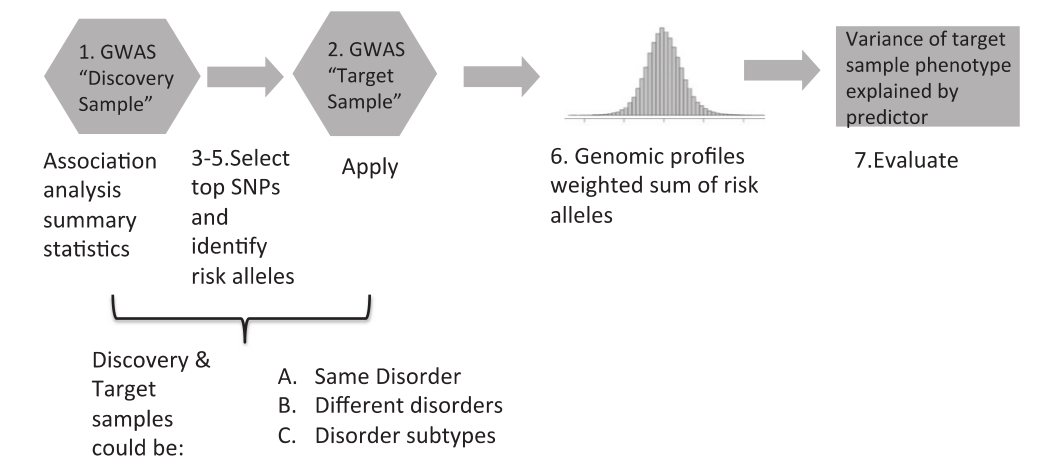
\includegraphics[width=0.8\textwidth]{genomic-profile.png}}
\caption{Illustration of the steps in genomic profile risk scoring. Source: \cite{wray2014research}.}\label{fig:steps-PRS}
\end{figure}

\begin{figure}[htb]
\centerline{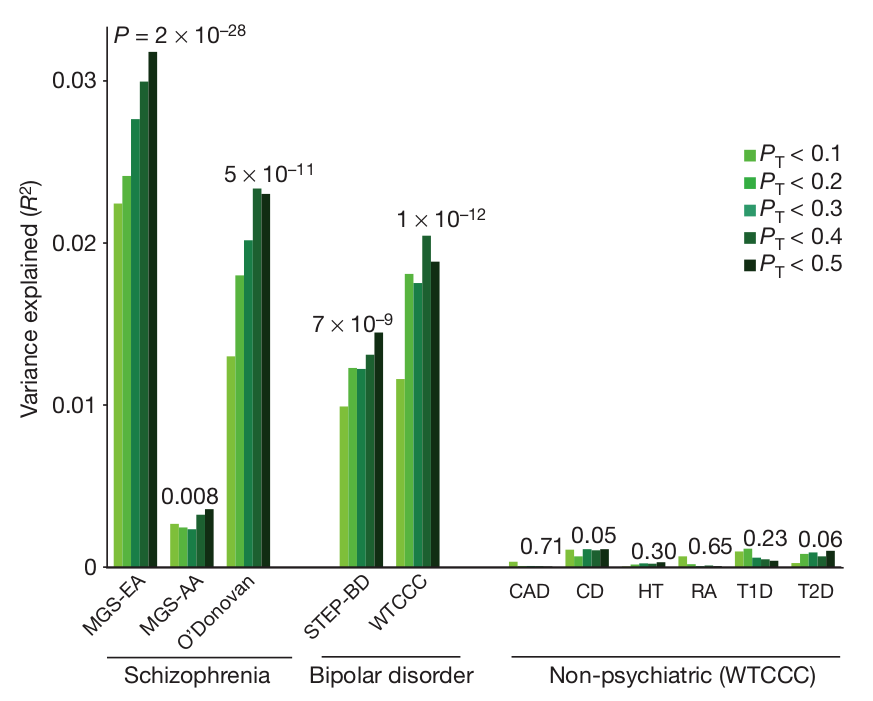
\includegraphics[width=0.65\textwidth]{purcell2009.png}}
\caption{Replication of the polygenic component derived by the International Schizophrenia Consortium in independent schizophrenia and bipolar disorder samples. A PRS was computed using summary statistics from a GWAS of schizophrenia, and this polygenic score was tested for association with schizophrenia, bipolar disorder and other diseases in independent datasets. This proved that there was a polygenic contribution to schizophrenia, a common genetic contribution between schizophrenia and bipolar disorder, but no apparent common genetic contribution between schizophrenia and other diseases such as coronary artery disease, Crohn's disease, hypertension, rheumatoid arthritis and diabetes. Associations were maximized for $p_T = 0.5$, i.e.\ including more than half of all SNPs. Source: \cite{purcell2009common}.}\label{fig:epi-PRS}
\end{figure}

Another use of PRS for epidemiology is to test the PRS for association with a phenotype that is different from the one used to compute the summary statistics.
This technique enables researchers to prove that there is a common genetic contribution between two traits. 
For example, it was shown that there is a common genetic contribution between Schizophrenia and bipolar disorder (Figure \ref{fig:epi-PRS}). 


\subsection{The differing goals of association testing and risk prediction}

Association testing (GWAS) and prediction have very different goals.
First, GWAS aims at identifying highly replicable disease-associated variants by using a highly stringent p-value threshold to prevent false discoveries. However, using only hits from GWAS results in PRS of low predictive value (see section \ref{sec:missing}). 
A common mistake is to report highly significant findings with large odds ratios as useful predictors of disease. 
Thus, people have been reminded over the years that GWAS findings are often not predictive on their own even if they are highly associated with the disease of interest, and that we would need scores that combine many SNPs in order to have a decent predictor of disease, i.e.\ polygenic scores \cite[]{pepe2004limitations,janssens2006predictive,jakobsdottir2009interpretation,wald2019illusion}.

Finally, it should be noted that population stratification, usually considered an unwelcome confounder in GWAS, may be useful in risk prediction and may be leveraged to produce better models \cite[]{golan2014effective,abraham2015genomic}.
Indeed, for predictive purposes, the objective is to provide the best possible prediction and confounding is not an issue. However, it might become an issue when polygenic risk scores (PRS) capture population structure in addition to trait variation. For instance, correlation between a PRS and an outcome might be due to residual population structure instead of real genetic contribution to the outcome \cite[]{sohail2019polygenic}.


\section{Polygenic prediction}

\subsection{Heritability and missing heritability} \label{sec:missing}

The basic components of disease risk are usually broken down into genetic susceptibility, environmental exposures and lifestyle factors. Thus, all disease incidence cannot be predicted by genetic factors only.
For a quantitative phenotype, we call heritability ($h^2$) the proportion of phenotypic variation that is attributable to genetic factors among a population \cite[]{visscher2008heritability}.
Methods now enable the estimation of chip-heritability (also called SNP-heritability: $h^2_{SNP}$) using linear mixed models and residual maximum likelihood. For example, for a chip of 300K SNPs, it was shown that those SNPs could account for 45\% of the variance of height \cite[]{yang2010common}.
Note that the heritability of height is estimated to be around 80\% \cite[]{silventoinen2003determinants,visscher2006assumption}; the difference between these two values can be explained by the fact that 300K SNPs cannot capture the same variation in height as the 3 billion base pairs of DNA. This difference can also reflect an overestimation of heritability \cite[]{visscher2008heritability}. Authors of a recent preprint claim that they can recover the full heritability for height and BMI using both rare and common variants from NGS data \cite[]{wainschtein2019recovery}.

So, basically, heritability is the upper bound in terms of prediction power (when measured with $R^2$) that we can get using a model from genetic variants only.
The difference between $R^2$ and $h^2$ has been termed ``missing heritability'' \cite[]{manolio2009finding}. So, the main goal of genetic prediction and my thesis is to get best possible predictions based on genetic data in order to reduce this missing heritability.

The gap between predictions and heritabilities was really huge in the first years of GWAS.
For example, first GWAS found only 12 associated SNPs for type 2 diabetes and only 2 for prostate cancer, explaining a very small proportion of heritability for these diseases \cite[]{jakobsdottir2009interpretation}. 
Likewise, in 2008, only 40 genome-wide-significant SNPs had been identified for height, and together these explained about 5\% of the heritability of height \cite[]{manolio2009finding}. In 2014, the number of associated SNPs had increased to around 700, explaining 20\% of the heritability of height \cite[]{wood2014defining}.
Since most of the identified associated SNPs have an effect size close to the limit dictated by the power of the studies, a likely explanation, at least in part, is that there are many common polymorphisms with effects that are too small to pass the stringent significance threshold of current GWAS \cite[]{wray2008prediction}.
Therefore, as results from multiple GWAS are combined to increase sample size, a larger fraction of the genetic variance is likely to be explained and accurate prediction of genetic risk to disease will become possible even though the risks conveyed by individual variants are small \cite[]{wray2008prediction,wray2018common}.
These findings have also led people to use not only genome-wide significant SNPs, but many other SNPs, sometimes not even marginally significant (i.e.\ with a p-value > 5\%) in order to maximize predictive power \cite[]{purcell2009common,Dudbridge2013,wray2014research}.


\subsection{Methods for polygenic prediction}

Several methods have been developed to predict disease status based on SNP information.
We can divide these methods in two categories: the ones that use summary statistics and the ones that use individual-level data only.

When summary statistics are available, the most widely used method is called ``Clumping + Thresholding'' (C+T), which has been described in section \ref{sec:C+T}.
More recently, researchers have focused their efforts on implementing more elegant and potentially more optimal ways to account for LD, as a replacement of clumping that simply discards SNPs \cite[]{vilhjalmsson2015modeling,mak2017polygenic,chun2019non,ge2019polygenic}. 
Take the solution of a linear regression $y = X \beta + \epsilon$, $\hat{\beta} = \left(X^T X\right)^{-1} X^T y$. This vector of effect sizes $\hat{\beta}$, estimated from all variables at once, can be decomposed in two parts: $X^T y$ that represents the marginal effects, i.e.\ the effects of each variable when learned independently; and $\left(X^T X\right)^{-1}$, some rotation of the effects that account for the correlation between variables.
Then, the first element can be replaced by summary statistics and the second element can be replaced by an estimation of the LD structure of the SNPs, e.g.\ from a reference panel. 
In practice, [$X^T y$ is estimated by TODO] and $\left(X^T X\right)^{-1}$ is computed by window. [TODO: parler de bayesian or lasso]


Moreover, these methods handle weights differently than C+T that directly uses GWAS effect sizes as weights in the PRS, or weights of 0 for SNPs not passing the thresholding step. Instead, these methods usually shrink effects towards 0. 
Apart from the method of \cite{mak2017polygenic}, the other methods do not perform variable selection at all. This means that if you use GWAS summary statistics for 10M variants as input, you would get a predictive model composed of 10M variables \cite[]{janssens2019polygenic}.

When using individual-level data only, the problem boils down to a standard classification problem. Thus, some statistical learning methods have been used to derive PRS for complex human diseases by jointly estimating SNP effects. Such methods include joint logistic regression, Support Vector Machine (SVM) and random forests \cite[]{wei2009disease,abraham2012sparsnp,abraham2014accurate,botta2014exploiting,okser2014regularized}.
Linear Mixed-Models (LMMs) are another widely-used method in fields such as plant and animal breeding or for predicting highly heritable quantitative human phenotypes such as height \cite[]{yang2010common}. 
However, these methods and their derivatives are often computationally very demanding, both in terms of memory and time required \cite[]{zhou2013polygenic,golan2014effective,speed2014multiblup,maier2015joint}.
Recently, two methods named BOLT-LMM and SAIGE have been developed to handle very large datasets \cite[]{loh2018mixed,zhou2018efficiently}. BOLT-LMM and SAIGE were primarily designed for association testing but could also be used for prediction purposes based on individual-level data.

\subsection{Objective and main difficulties of the thesis}

We want to use genetic data to help distinguish between cases and controls for a given disease, or at least to stratify people in the population in order to improve early detection of diseases and prevention for high-risk individuals.
Genomic data are usually very large and highly dimensional with hundreds of thousands of variables to many millions, for thousands or hundred of thousands individuals.
Thanks to large sample sizes of recent GWAS studies, many robust associations between DNA variants and many diseases have been identified. Yet, individually, these variants generally have a small effect on disease susceptibility, explaining a small fraction of the total heritability of the diseases studied. 
In order to have predictive models useful in clinical settings, we need to combine the information from a multitude of DNA variants, coming from multiple studies, and in diverse formats (e.g.\ individual-level data and summary statistics).

To improve current disease predictions from Polygenic Risk Scores (PRS), we have focused on using methods from the statistical learning community, which have received only moderate attention in the "predictive human genetics" field.
The main difficulty in using these methods is that they do not necessarily scale well with the large-scale data we now have in this field.
For example, the UK Biobank is composed of 500K individuals from which 90M variants are available \cite{bycroft2017genome}.
When analyzing these large-scale datasets, only a few methods are usable.
Most of them are being developed in a separate piece of software that does a specific analysis.
Yet, if you want to do some exploratory analyses and test new ideas, it becomes increasingly difficult to do so.

Thus, the first part of our work has been dedicated to developing two R packages that could handle very large datasets, while being simple and flexible to use for both standard and exploratory analyses. 
Our second paper has been dedicated to implementing penalized regressions as a replacement to more simple, less optimal methods, and that could be used for very large individual-level datasets.
Finally, because lots of summary statistics data are available while individual-level data are still scarce, we worked on making the most out of the Clumping and Thresholding (C+T) method since it proved to be a simple and effective method for constructing PRS based on large GWAS summary statistics and smaller individual-level datasets.
